\documentclass[a4paper,12pt]{report}

% Работа с русским языком
\usepackage{cmap}
\usepackage[utf8]{inputenc}
\usepackage[T2A]{fontenc}
\usepackage[english,russian]{babel}

\usepackage{amsmath,amsfonts,amssymb,amsthm,mathtools}
\usepackage{csquotes}
\usepackage{graphicx}
\usepackage{float}
\usepackage{icomma}

\usepackage{euscript}
\usepackage{mathrsfs}

\graphicspath{{./images/}}

\usepackage[nottoc]{tocbibind}

\usepackage{listings}

\lstdefinestyle{mystyle}{
  breakatwhitespace=false,         
  breaklines=true,                 
  captionpos=b,                    
  keepspaces=true,                 
  numbers=left,                    
  numbersep=5pt,                  
  showspaces=false,                
  showstringspaces=false,
  showtabs=false,                  
  tabsize=2
}

\lstset{style=mystyle}


\author{
	Малов Андрей\\
	\and
	Школьник Савелий\\
	\and
	Магомедрасулов Курбан\\
	\and
	Богатиков Валерий\\
}
\title{Нечёткая логика}
\date{\today}

\begin{document}
	
\maketitle

\tableofcontents

\chapter{Введение}

\section{Определение нечёткой логики}

\textbf{Нечёткая логика} --- это форма многозначной логики, в которой истинностными значениями переменных могут быть любые вещественные числа от 0 до 1 включительно. Она используется для обработки концепции частичной истины, где значение истины может колебаться между полностью истинным и полностью ложным. В отличие от булевой логики, где значениями переменных могут быть только целочисленные значения 0 или 1.

Термин нечёткая логика был введён в 1965 году в теории нечётких множеств Лотфи Заде. Хотя нечёткая логика изучалась с 1920-х годов как бесконечнозначная логика, особенно Лукасевичем и Тарским.

Нечёткая логика основана на наблюдении, что люди принимают решения на основе неточной и нечисловой информации. Нечёткие модели или наборы являются математическим средством представления неопределённости и неточной информации (отсюда и термин нечёткий). Эти модели обладают способностью распознавать, представлять, манипулировать, интерпретировать и использовать данные и информацию, которые являются расплывчатыми и недостоверными.

Нечёткая логика применяется во многих областях, от теории управления до искусственного интеллекта.

\section{Общее представление нечёткой логики}
Классическая логика допускает только те выводы, которые либо истинны, либо ложны. Однако существуют также предложения с переменными ответами, например, если попросить группу людей определить цвет. В таких случаях истина появляется в результате рассуждения на основе неточного или частичного знания, в котором отобранные ответы отображаются на спектре.

Обе степени истинности и вероятности находятся в диапазоне от 0 до 1 и поэтому могут показаться похожими на первый взгляд, но нечёткая логика использует степени истинности как математическую модель \textit{неопределённости}, в то время как вероятность - это математическая модель \textit{незнания}.

\subsection{Применение истинных значений}
Базовое приложение может характеризовать различные поддиапазоны непрерывной переменной. Например, измерение температуры для АБС тормозов может иметь несколько отдельных функций принадлежности, определяющих определённые температурные диапазоны, необходимые для правильного управления тормозами. Каждая функция отображает одно и то же значение температуры в диапазоне от 0 до 1. Эти значения истинности могут затем использоваться, чтобы определить, как следует управлять тормозами.

\subsection{Лингвистические переменные}
В то время как переменные в математике обычно принимают числовые значения, в нечёткой логике нечисловые значения часто используются для облегчения выражения правил и фактов.

Лингвистическая переменная, \textit{возраст} может принимать такие значения, как \textit{молодой}, так и его антоним \textit{старый}. Поскольку естественные языки не всегда содержат достаточное количество ценностных терминов, чтобы выразить нечёткую шкалу значений, общепринятой практикой является изменение лингвистических значений с помощью прилагательных или наречий.

Операции фаззификации могут отображать математические входные значения в нечёткие функции принадлежности. А противоположные операции де-фаззификации могут быть использованы для отображения нечёткой выходной функции принадлежности в \textquote{чёткое} выходное значение, которое затем может быть использовано для целей принятия решений или управления.

\section{Процесс}
\begin{enumerate}
	\item Привести все входные значения к нечётким функциям принадлежности.
	\item Выполнить все применимые правила в базе правил для вычисления нечётких выходных функций. 
	\item Де-фаззифицировать нечёткие выходные функции, чтобы получить \textquote{чёткие} выходные значения.
\end{enumerate}
\subsection{Фаззификация}
Фаззификация - это процесс присвоения числовых входных данных системы нечётким множествам с некоторой степенью принадлежности. Эта степень принадлежности может быть задана в пределах интервала [0,1]. Если она равна 0, то значение не принадлежит данному нечёткому множеству, а если равно 1, то значение полностью принадлежит нечёткому множеству. Любое значение в диапазоне от 0 до 1 представляет собой степень неопределённости того, что это значение принадлежит множеству. Эти нечёткие множества обычно описываются словами, и поэтому, назначая входные данные системы нечётким множествам, мы можем рассуждать о них лингвистически естественным образом.

Например, на рисунке ниже значения выражений \textit{холодный}, \textit{тёплый} и \textit{горячий} представлены функциями, отображающими шкалу температуры. Точка на этой шкале имеет три \textquote{истинностных значения} --- по одному для каждой из трёх функций. Вертикальная линия на изображении представляет собой определённую температуру, которую измеряют три стрелки (истинные значения). Поскольку красная стрелка указывает на ноль, эта температура может быть интерпретирована как \textquote{не горячая}, т. е. эта температура имеет нулевое членство в нечётком множестве \textquote{горячая}. Оранжевая стрелка (указывающая на 0.2) может описать его как \textquote{слегка тёплый}, а синяя стрелка (указывающая на 0.8) --- как \textquote{довольно холодный}. Следовательно, эта температура имеет 0,2 членства в нечётком множестве \textquote{тёплый} и 0,8 членства в нечётком множестве \textquote{холодный}. Степень принадлежности, присвоенная каждому нечёткому множеству, является результатом размытия.

\begin{figure}[H]
	\centering
	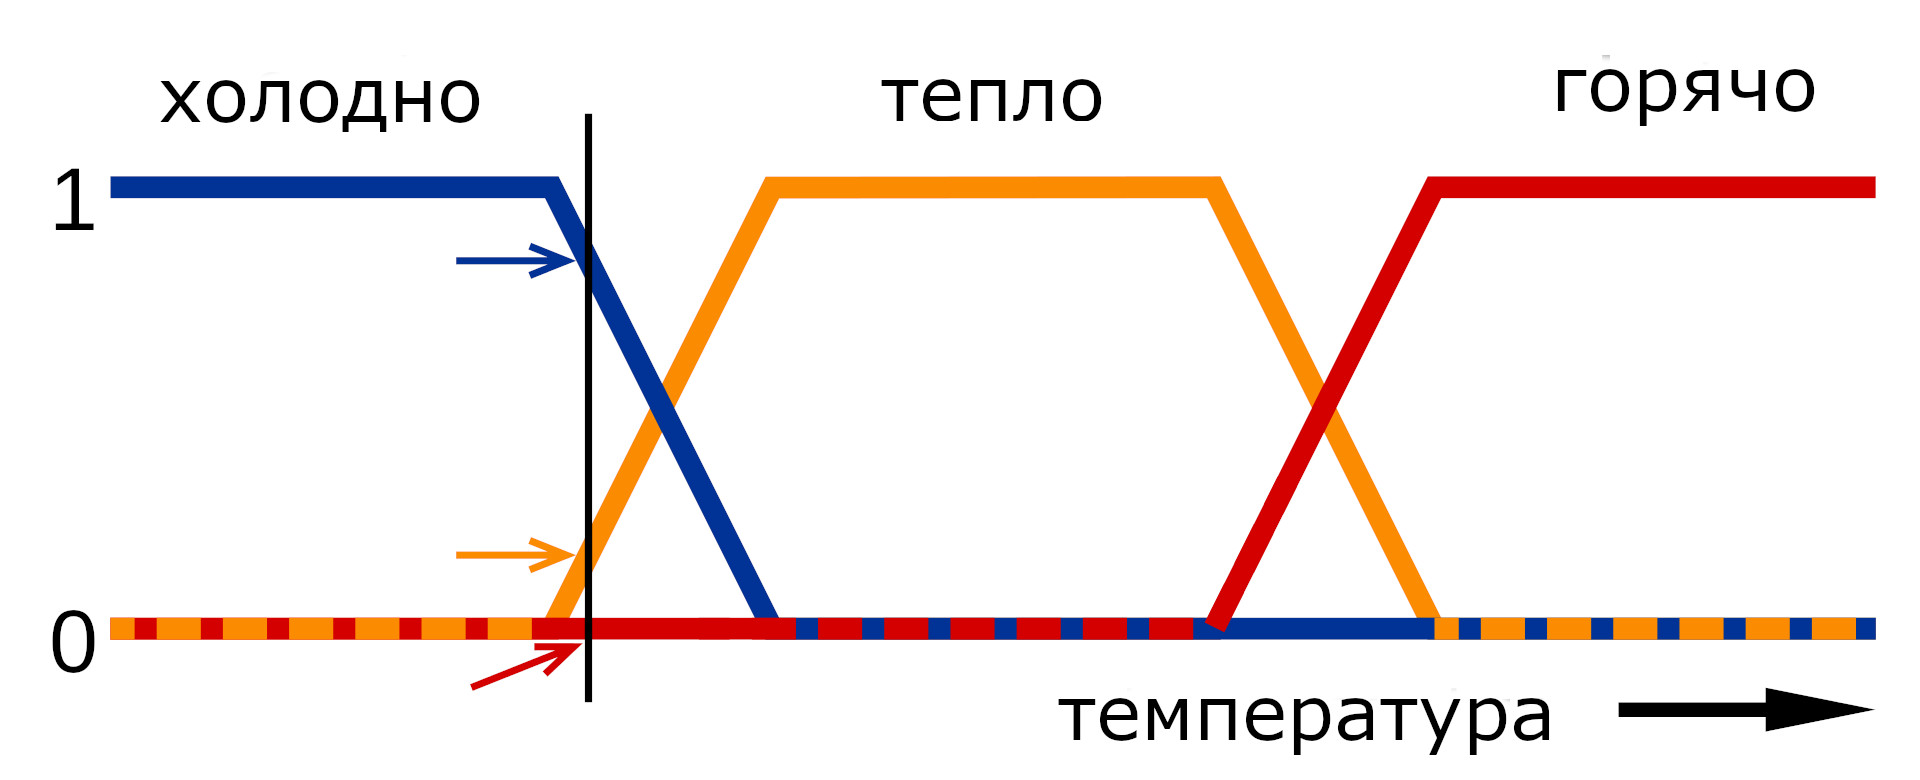
\includegraphics[width=0.5\textwidth,keepaspectratio]{images/temp_example.jpg}
	\caption{Температура нечёткой логики}
\end{figure}

Нечёткие множества часто определяются как треугольные или трапециевидные кривые, наклон может быть, если значение увеличивается, пик, там где значение равно 1 (который может иметь длину 0 или больше) и наклон, где значение уменьшается. Они также могут быть определены с помощью сигмоиды. Одним из распространённых случаев является стандартная логистическая функция, определяемая как

\[S(x) = \frac{1}{1 + e^{-x}}\]

которая обладает следующим свойством симметрии

\[S(x) + S(-x) = 1\]

Из этого следует, что

\[(S(x)+S(-x))*(S(y)+S(-y))*(S(z)+S(-z)) = 1\]

\subsection{Операторы нечёткой логики}
Нечёткая логика работает со значениями принадлежности таким образом, что имитирует Булеву логику. С этой целью должны быть доступны замены для основных операторов И, ИЛИ, НЕТ. Для этого есть несколько способов. Распространённая замена называется \textit{операторами Заде}:

\begin{center}
	\begin{tabular}{ |c|c| }
		\hline
		\textbf{Булева логика} & \textbf{Нечёткая логика}  \\
		\hline
		\(AND(x, y)\) & \(MIN(x, y)\)  \\
		\hline
		\(OR(x, y)\) & \(MAX(x, y)\)  \\
		\hline
		\(NOT(x)\) & \(1 - x\)  \\
		\hline
	\end{tabular}
\end{center}

Для TRUE/1 и FALSE/0 нечёткие выражения дают тот же результат, что и логические выражения.

Однако таблица произвольного выбора не всегда определяет функцию нечёткой логики. Был сформулирован критерий для определения того, определяет ли данная таблица выбора функцию нечёткой логики, и был предложен простой алгоритм синтеза нечёткой логической функции, основанный на введённых понятиях составляющих минимума и максимума. Функция нечёткой логики представляет собой дизъюнкцию составляющих минимума, где составляющая минимума представляет собой совокупность переменных текущей области, большей или равной значению функции в этой области (справа от значения функции в неравенстве, включая значение функции).

Другой набор операторов И/ИЛИ основан на умножении\\

\(x\) AND \(y\) = \(x*y\)

\(x\) OR \(y\) = \(1-(1-x)*(1-y) = x+y-x*y\)\\
	

\(1-(1-x)*(1-y)\) исходит из этого:\\

\(x\) OR \(y\) = NOT(AND(NOT\((x)\), NOT\((y)))\)

\(x\) OR \(y\) = NOT(AND\((1-x, 1-y) )\)

\(x\) OR \(y\) = NOT\(( (1-x)*(1-y) )\)

\(x\) OR \(y\) = \(1-(1-x)*(1-y)\)

\subsection{Правило ЕСЛИ-ТО}
Правила ЕСЛИ-ТО сопоставляют входные или вычисленные значения истинности с требуемыми выходными значениями истинности. Пример:\\

ЕСЛИ температура \textit{очень холодная}, ТО скорость вращения вентилятора \textit{останавливается}

ЕСЛИ температура \textit{холодная}, ТО скорость вращения вентилятора \textit{медленная}

ЕСЛИ температура \textit{тёплая}, ТО скорость вращения вентилятора \textit{умеренная}

ЕСЛИ температура \textit{горячая}, ТО скорость вращения вентилятора \textit{высокая}\\

При определённой температуре нечёткая переменная \textit{горячий} имеет определённое значение истинности, которое копируется в переменную \textit{высокая}.

\subsection{Дефаззификация}
Цель состоит в том, чтобы получить непрерывную переменную из нечётких истинностных значений.

Это было бы легко сделать, если бы выходные истинностные значения были точно такими же, как и те, которые получены в результате фаззификации данного числа. Однако, поскольку все выходные значения истинности вычисляются независимо, в большинстве случаев они не представляют такой набор чисел. Затем нужно выбрать число, которое лучше всего соответствует \textquote{намерению}, закодированному в значении истинности. Например, для нескольких истинностных значений \textit{скорости вращения вентилятора} необходимо найти фактическую скорость, которая наилучшим образом соответствует вычисленным истинностным значениям переменных \textquote{медленный}, \textquote{умеренный} и т. д.

Для этой цели не существует единого алгоритма.

Общий алгоритм таков:
\begin{enumerate}
	\item Для каждого значения истинности сократите функцию принадлежности на это значение
	\item Объедините полученные кривые с помощью оператора OR
	\item Найдите центр тяжести области под кривой
	\item Позиция \(x\) этого центра является окончательным выводом.
\end{enumerate}

\section{Формирование консенсуса входных данных и нечётких правил}
Поскольку вывод нечёткой системы является консенсусом всех входов и всех правил, системы нечёткой логики могут хорошо себя вести, когда входные значения недоступны или не заслуживают доверия. Весовые коэффициенты могут быть дополнительно добавлены к каждому правилу в базе правил, также весовые коэффициенты могут использоваться для регулирования степени влияния правила на выходные значения. Эти весовые коэффициенты могут основываться на приоритете, надёжности или согласованности каждого правила. Эти веса правил могут быть статическими или могут изменяться динамически, даже на основе выходных данных других правил.

\section{Первое применение}
Многие из ранних успешных применений нечёткой логики были реализованы в Японии. Первое известное применение это --- метро в Сендай, в котором нечёткая логика была в состоянии улучшить экономичность, комфорт и точность поездки. Нечёткая логика также используется для распознавания рукописных символов в карманных компьютерах Sony, для помощи в полете для вертолётов, для управления системами метрополитена с целью повышения комфорта при вождении, точности остановки и экономии энергии, повышения расхода топлива для автомобилей, управление одной кнопкой для стиральных машин, автоматическое управление двигателем для пылесосов с распознаванием состояния поверхности и степени загрязнения, а также системы прогнозирования для раннего распознавания землетрясений через Институт сейсмологии Бюро метеорологии, в Японии.

\chapter{Программная часть}
\section{Выбор инструмента}
Задача состоит в том, чтобы составить программу для...
\section{Программа на Python}
\lstinputlisting[language=Python, caption=Полная программа на Python]{../main.py}


\chapter{Заключение}
В заключение хочется отметить, что нечёткая логика всё активнее используется в разных областях нашей жизни. В середине 1970-х гг. были предложены первые реализации нечётких моделей в промышленности, а в начале 1980-х гг. нечеткая математика получила свое дальнейшее развитие в целом ряде программных средств поддержки принятия решений и в экспертных системах анализа данных.

В настоящее время приложения нечеткой математики можно найти в сотнях промышленных изделий — от систем управления электропоездами и боевыми вертолетами до бытовой техники. Нечеткая логика используется для принятия политических решений и моделирования возможных кризисных ситуаций в современных ситуационных центрах руководителей западных стран, в программных системах, обслуживающих большой бизнес. Например, компания Yamaichi Securities на основе нечёткой логики разработала интеллектуальную банковскую систему для средне и долгосрочных операций с корпоративными бумагами системы.

Нечеткой логике обязано своим рождением и новое поколение систем имитационного моделирования. Большинство программных комплексов, используемых в мире для экономического, политического и финансового моделирования, базируется на методах динамики систем (system dynamics). Системная динамика — это метод имитационного моделирования, основанный на представлении системы на высоком уровне абстракции как совокупности потоков, накопителей, вспомогательных переменных и субмоделей со своими элементами.

В последнее время нечеткое управление является одной из самых активных и результативных областей исследований применения теории нечетких множеств. Нечеткое управление оказывается особенно полезным, когда технологические процессы являются слишком сложными для анализа с помощью общепринятых количественных методов, или когда доступные источники информации интерпретируются качественно, неточно или неопределенно. Экспериментально показано, что нечеткое управление дает лучшие результаты, по сравнению с получаемыми при общепринятых алгоритмах управления.

Нечеткие методы помогают управлять домной и прокатным станом, автомобилем и поездом, распознавать речь и изображения, проектировать роботов, обладающих осязанием и зрением. Нечеткая логика, на которой основано нечеткое управление, ближе по духу к человеческому мышлению и естественным языкам, чем традиционные логические системы. Нечеткая логика, в основном, обеспечивает эффективные средства отображения неопределенностей и неточностей реального мира. Наличие математических средств отражения нечеткости исходной информации позволяет построить модель, адекватную реальности.

\bibliographystyle{unsrt}
\bibliography{sample}


\end{document}
